\documentclass[../main.tex]{subfiles}
 
\begin{document}

\section{Monday}

In the morning, you attempt to sit through Nvidia's Vulcan presentation. From the website:

\begin{quote}
Vulkan is a modern cross-platform graphics and compute API currently in development by the Khronos consortium.
\end{quote}

It sounds cool when you read \textit{Vulcan} in your little schedule. Perhaps this will be your first technical talk that streches your brain a bit. You're ready for some mental gymnastics. This is the kind of thing you were hoping for. Food for the brain. A lecture that will introduce you to something you can take back with you and investigate further. You meet a coworker seated behind you and settle in for a technical talk which you figure may introduce you to some GPU fundamentals. You are mistaken. Instead, you are treated to slides averaging no less than 200 words, not counting the ones which literally show hundreds of lines of unintelligible source code. Okay, perhaps for some in the audience what is presented makes perfect sense, but you feel the creeking and sighs of folks shifting in their seats around you and you can almost imagine the wheels in people's heads grinding and thudding to a halt. This is \textit{bad}. This is not how you present, you think to yourself. You actually think back to your last semester of undergrad, during which you had the privelage of taking a public speaking class, which you adored. You gave a TED talk to your class about your attitude towards math and three mentors who had a big impact on you. This is what you daydream about as the speaker drones on. \textit{This} is what you were warned against. No matter who your audience is, this cannot possibly be the best way to impart technical knowledge. This is torture. You are presented with diagram after diagram, none of which make any sense to you. You excuse yourself after 40 minutes of this to head down to VR village after wondering about Experience Hall. It had been your intention to spend less time looking at the smoke and mirrors in Experience Hall and more time pondering the material of the technical talks. You'll have to study the programming a bit more next time before you waltz into another talk like this. On your first day at SIGGRAPH, you worked with the Japanese haptic technology lab. Now you would like to experience Emerging Technology (E-Tech) from an attendees perspective. A walk through Experience Hall lets your brain cool off after the Vulcan meltdown.

You try the HapticWave demonstration at the Oculus booth, which is stationed next to the booth you where you worked the previous day. The Occulus demonstration is wholly more convincing and polished than the work done by the Japanese lab you assisted during your first shift just one booth over. While standing in line you read the two page handout which attemps to outline the main advancements made by this particular haptic technology. A thin metal plate sandwhiching a ring of magnets will trick you into perceiving a ball's position as it bounces around a virtual table in front of you. This is the first time you have ever tried an Occulus headset, let alone their latest model sporting higher resolution and fewer visual artifacts thought to detract from the immersive experience. Despite the obvious technical advancements being demonstrated throughout a large portion of Experience Hall, you can't help but be less than enthusiastic about all of this VR stuff. Here's why: their's no emotion. Most of these demonstrations are technical and do not incorporate cute characters, interesting plot, or convincing human interaction.

You then wander about the rest of the Experience Hall, growing increasingly jaded with the new technologies. You decide what you want out of SIGGRAPH are technical talks pitched at an appropriate level and the opportunity to hear \textit{behind the scenes} talks from the folks who know how to tell stories. The technology fest in E-Tech is simply overwhelming and does not seem to be worth investing your time in. That being said, your next shift has you helping a researcher named David Zielinski who works at the college you just graduated from. You recognize him and are happy to help out with a virtual archeology simulation which lets people explore a site in Spain simply by looking down at a virtual clipboard in their hand and searching for items which satisfy the checklist it maintains. This simulation happens to be created by a collaboration between your alma mater and University of São Paulo. The user interface is far from perfect, with attendees often getting lost or confused as to how they should proceed. Everyone who tries the simulation, yourself included, is absolutely amazed by the display. You begin to see the educational value of VR and appreciate the natural beauty of the virtual site, which was created not by talented modelers, but instead by photogrammetry from high resolution photos taken of an inaccessible site with archeological significance.

After this shift with David, you are preparing to get a ticket for the Monday Computer Animation Festival. Also known as \textit{Electronic Theater}, this show will be run twice during SIGGRAPH on both Monday and Wednesday evening. When you went to the Student Volunteer office in the morning to check in for the day's first shift, you inquired about getting your free ticket. Unfortunatlely, you were informed that only a Wednesday ticket is available. You take the ticket and hope to swap with another student, making a desparate post to the SV Facebook group asking for someone to bail you out. By the time the showtime rolls around, you are intending to try your luck at following your friend in line and hoping the SV responsible for checking tickets doesn't bother to read the date on your ticket. You are not this lucky when you are denied entrance by a fellow student volunteer at the entrance. After waiting in line for 20 minutes, you are instructed to leave the line that is now about 700 deep to run to the opposite end of the convention center to swap your Wednesday ticket for a Monday ticket. And you do run. You eventually make it inside and, hilariously, end up being ushered to a seat in the second row. This will turn out to be one of the most visually impressive places to experience the show, as well as the most accoustically traumatic. The bass literally blows your hair around throughout the show. You find this both uncomfortable and totally awesome.

The Computer Animation Festival is truly a special event. Lasting from 6 to 8pm, you are treated thorughout to award-winning student films, reels by companies like MPC showcasing their state-of-the-art rendering, and finally shorts by Disney and Pixar that truly steal the show. Disney's short called \textit{Inner Workings} is being exclusively shown at SIGGRAPH, so you are eager to see a glimpse at work that is not avaiable to the genral public. The full rundown of CAF is as follows:

\begin{enumerate}
	\item \textit{Accidents, Blunders and Calamities} --- a hilarious depiction of inventive ways for animals and insects to meet their demise.
	\item \textit{Tea Time} --- A grandma and her robot. Very French with an odd art style.
	\item \textit{Alike} --- One of several shorts aimed at showing how much work and failing to march to the beat of your own drum can be a real drag. 
	\item \textit{Tokyo Cosmo} - A dreamlike sequence for a young girl living in Japan.
	\item \textit{Glass Half} --- Absolutely phenomenal animation by the Blender Foundation.  A clever, colorful 2D cartoon using nonsensical vocalizations in the voice acting to push the audience into constant fits of laughter.
	\item \textit{Citipati} --- A dinosaur and a meteor. Lifelike rendering.
	\item \textit{Natural Attraction} --- The drama of a volcanic eruption unfolds in fantastic detail. Highly realistic physical rendering. Like watching an IMAX movie of a real eruption with impossible timelapse cinematography and angles, all done with CG. I felt chills watching this.
	\item \textit{League of Legends: Project Overdrive} --- The art style was bananas.
	\item \textit{Solar Superstorms} --- An example of animation based off fantastically complex simulations. This demonstration emphasizes a need for real-time data-visualization used for physics simulations, a topic that will be presented at a Nvidia talk at the end of the week.
	\item \textit{Mafia III} --- Video games are getting pretty (gruesome).
	\item \textit{Lichtspiel} --- A mindblowing intro sequence for a film festival .
	\item \textit{Terminator Genisys} --- MPC showing off.
	\item \textit{Behind The Magic: Warcraft} --- Industrial Light \& Magic showing off.
	\item \textit{Les marmottes: Mariachi} --- Hilariously placed between other longer shorts. 10 seconds of marmottes playing instruments, uh, realistically.
	\item \textit{Behind The Magic: Marvel's Captain America: Civil War} --- Layered effects.
	\item \textit{Crabe-Phare} --- Best Student Project award winner and my absolute favorite film that wasn't Pixar's \textit{Piper}.
	\item \textit{Shell V-Power Shapeshifter} --- A really involved automotive commercial with a behind the scenes look at the monster that was created for the TV spot.
	\item \textit{Borrowed Time} --- One of those films that raises the bar for story telling in animation. Winner of Best in Show.
	\item \textit{Escargore} --- Slugs. Funny in the way \textit{Accidents, Bludners and Calamities} was refreshing and full of physical comedy. Lots of smashing, burning, chopping, and exploding.
	\item \textit{Cosmos Laundromat} --- The soundtrack alone gave me chills. This is part of work in progress that is strangely released under Creative Commons by the Blender Foundation. You watch this a few more times on Youtube after returning from SIGGRAPH.
	\item \textit{Taking Flight} --- Good like \textit{Toy Story} is good.
	\item \textit{Moana} --- Sneak peek at an upcomming Disney film.
	\item \textit{None of that} --- Ringling College of Art and Design.
	\item \textit{Inner Workings} --- I've got a poster of this short at my desk at work.
	\item \textit{Piper} --- So cute. The rendering is as mind blowing as the elegance of the story. No dialogue, just a little bird that overcomes fear.
\end{enumerate}

After Computer Animation Festival, you make your way to a reception held out in front of the convention center. WIth you ticket, you are allowed as much food as you want from the dozens of food trucks parked on either side of tables and chairs lined along the pavement between palm trees. With your new friends Jen and Diede you make your way around the food trucks and head towards the beer and wine dispenseries to use your free drink ticket. While in line for your Anaheim Gold, thre three of you start to talking with a nice gentleman in line behind you wearing a shirt with \textit{Google} formed by a tesselation of triangles. As you get to talking, you find out that he works as an engineer on self-driving cars in the Mountain View office. Specifically, he works in graphical tools and rendering for user interfaces that will be found in the cars. Before you know it, your friends have floated elsewhere and left you to talk for 20 minutes with the engineer from Google. His badge says \textit{Philip Nemec}. As it turns out, the product manager working on self-driving cars that you met at a summer writing program---the very same woman who kindly submitted the internal candidate referral which saw you pass a coding test and then complete a phone screening with Google before politely withdrawing your candidacy to accept your current job---well, it turns out she sits two desks over from this gentlemen. He's amused to hear Min Li Chan's name come up and you figure this alone may guarantee that you might hear back from him should you reach out to him after the event.

The two of you talk and you ask him a your new favorite question to pose to people like him: people who have been there and done that and might be willing to put down some sign posts for you. You prefer to ask not what he studied in college (computer science at Carnegie Mellon), but instead ask what he studied in the years right after college in order to bridge the gap between his formal education and what he needed to start moving towards what he is currently working on.


\begin{figure}[h!]
	\centering
	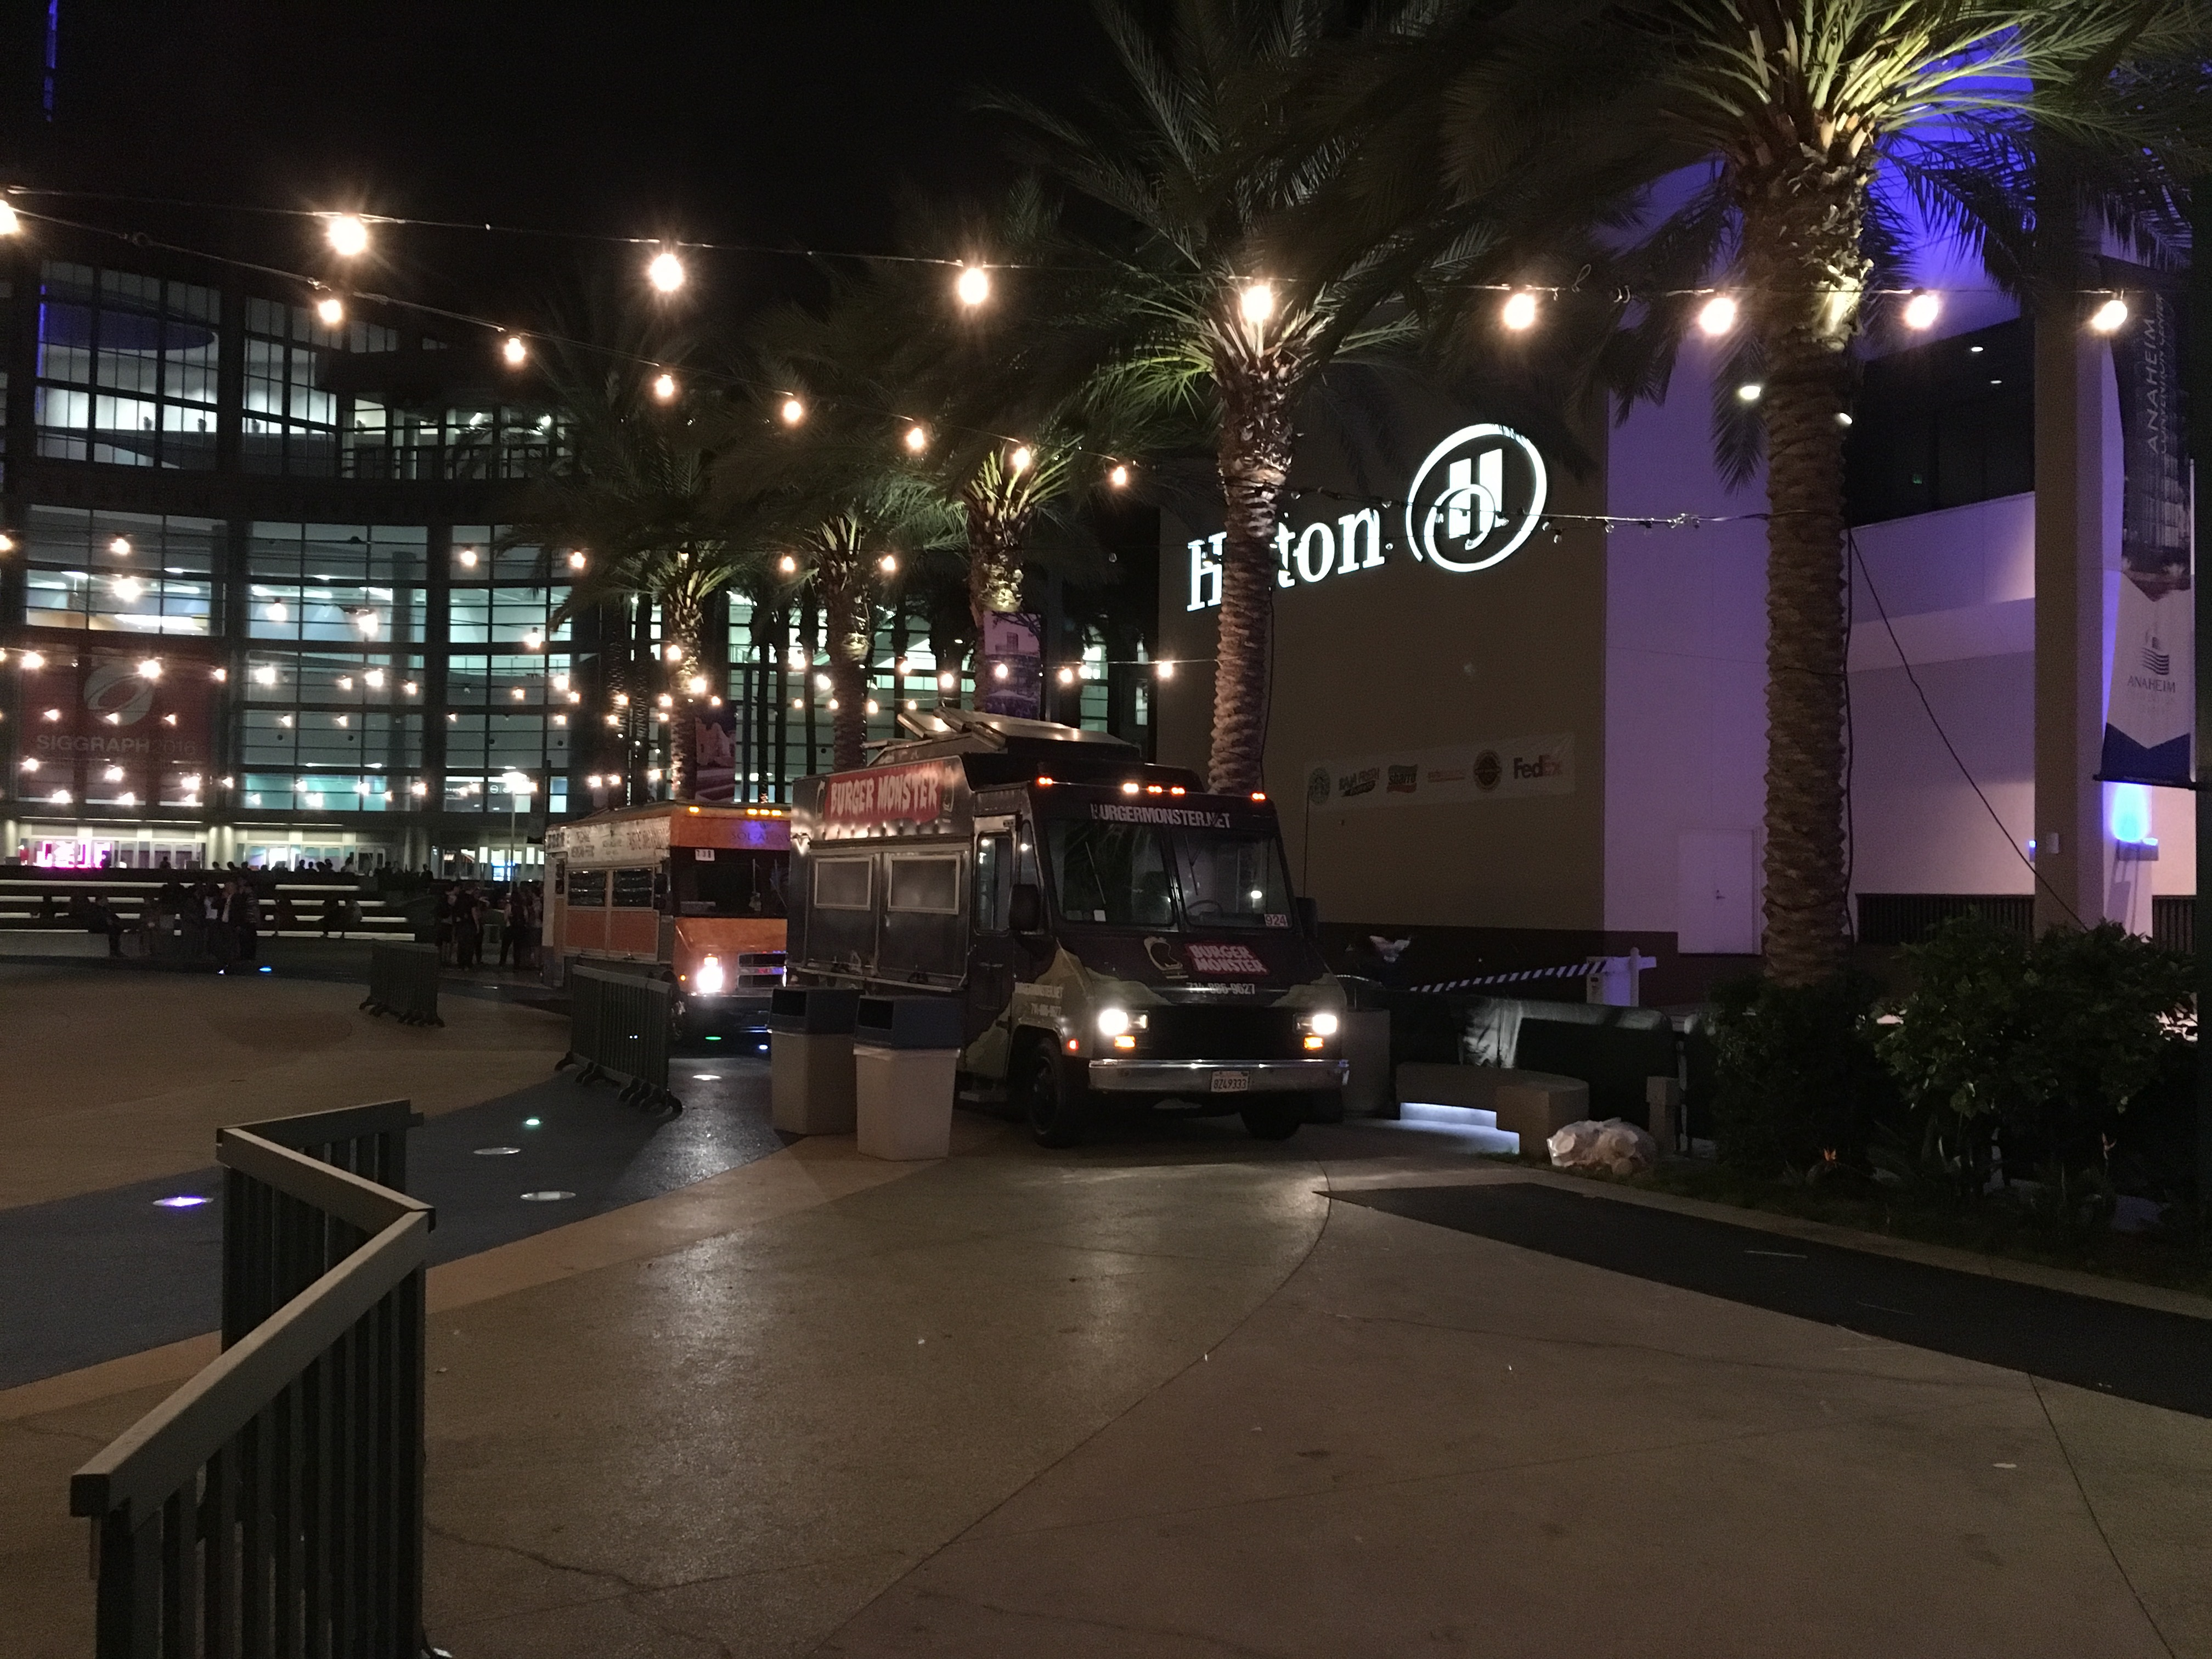
\includegraphics[width=\textwidth]{food_trucks}
	\caption*{SIGGRAPH 2016 Reception}
\end{figure}

Philip stresses the importance of picking little projects to dive deep into, using the example of becoming really knowledgeable about, say, typography and kerning. He also encourages you, with respect to your continuted math education that you suggest you will pursue in a self-study capacity for now, to learn more about probability and statistics. You show him a recent screenshot from a geometry library you wrote and talk about how as humble as that project really is, it was still complex in comparison to anything you had done before and taught you a great deal about organizing a big project into small, bite-sized pieces. In total its 1,000 lines of code, but from those 1,000 lines you learned some patterns which you figure might help you in projects of much greater scale. You tell him that you're biggest concern as you start out as a software engineer is becoming more mature in your approach to tackling big problems. You see this as a \textit{meta} skill which envelops other sharpened abilities which you might pick up from studying, say, discrete math or analysis or topology. There's learning to think logically---that's programming. Then there's learning to think translationally---that's what Justin Curry, Paul Bendich, and Chris Tralie have gotten better at by doing math. And then there's the ability to create organization from chaos which you imagine a high level software engineer has learned to do where other smart folks have the horsepower, but not the foresight and experience to do the same. 

\begin{figure}[h!]
	\centering
	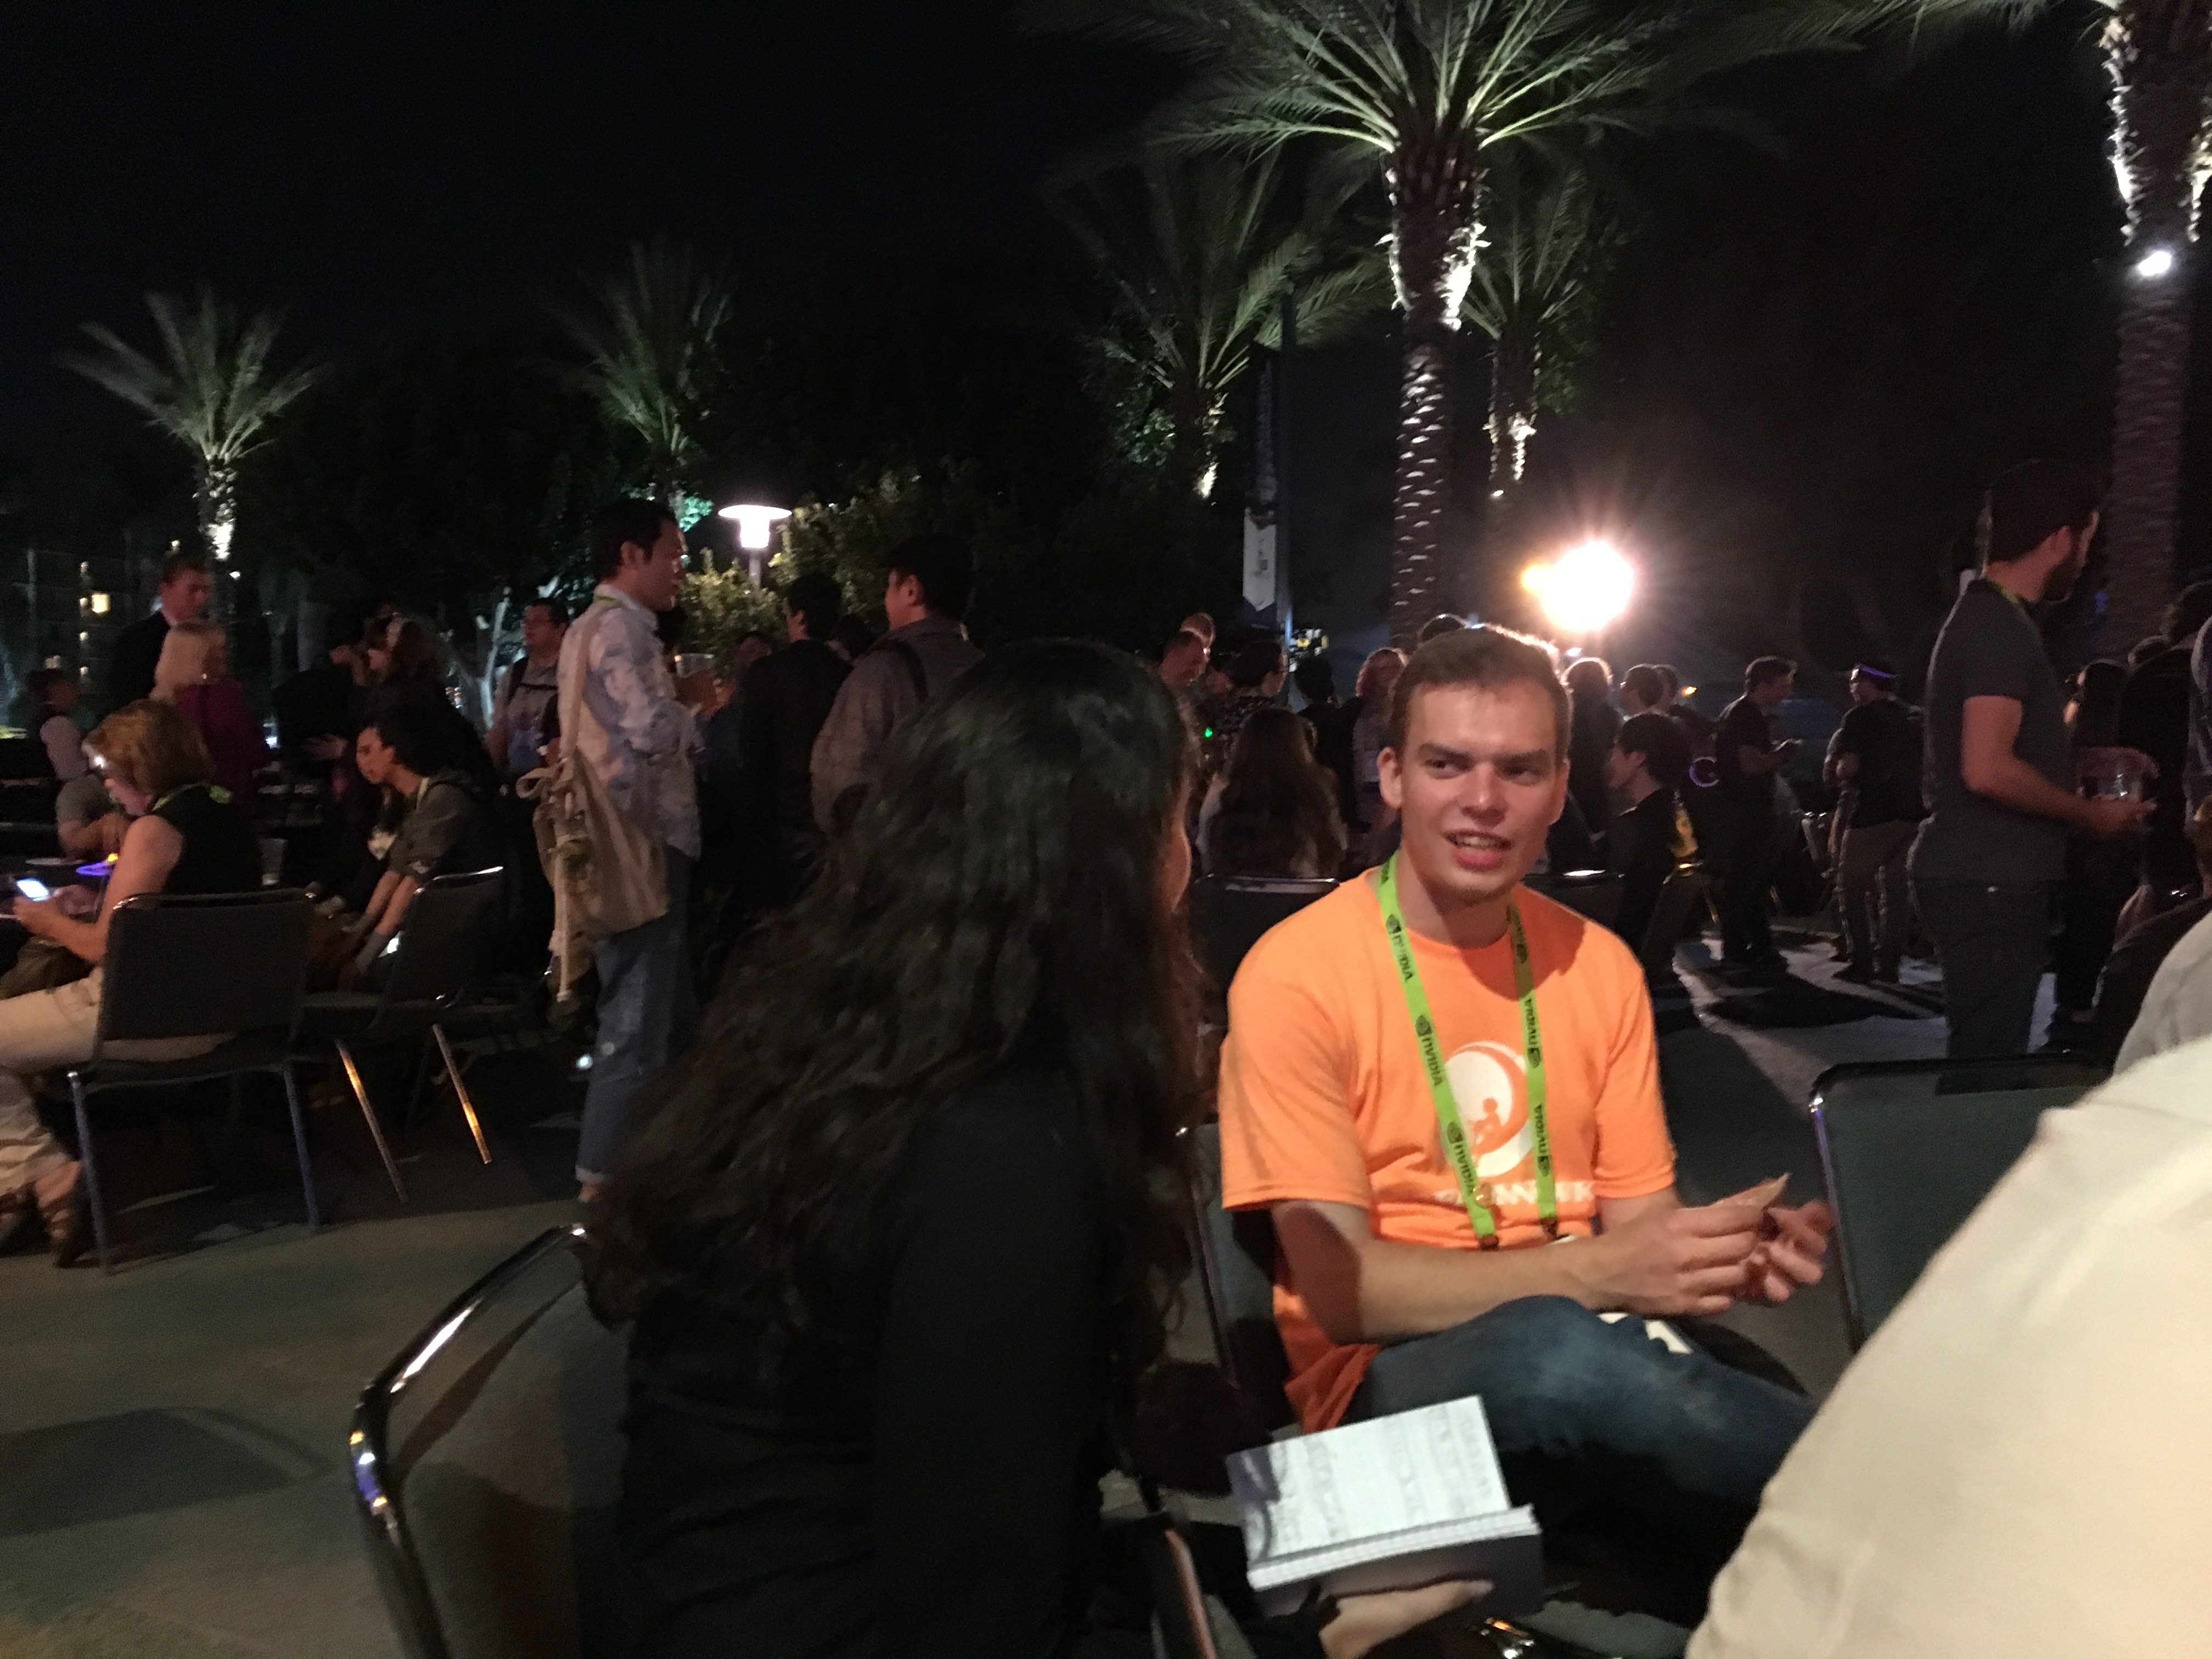
\includegraphics[width=\textwidth]{jen_diede}
	\caption*{Jen and Diede}
\end{figure}

How would one go about starting to build a CAD program from scratch? You mention your having read \textit{The Autodesk File} by John Walker, and Philip writes this down in his notebook while you are standing there besides the outdoor bar. You have'nt a very clear idea of how to break significant, open-ended research problems into a maintainable codebase. How would you go about laying out the groundwork for a self-driving car's core artificial intelligence codebase so that it might develop as painlessly as possible over the next 10 years? It is the ability to write code which might be reasoned about in a mathematical way and which might inspire confidence in its ability to provide lasting solutions long into the future that you intend to develop over the next few years. This isn't what they teach you in school---at least not at your school. You're going to have to learn this on the job and by contuning to follow bright folks who manage to both pave the way and show the world how they did it. Michael Abrash and Mike Bostock come to mind. You will continue to find resources and attempt to dive deep.

Philip takes a picture of your badge and hands you a business card. Again, your small oversite in not printing your own is mildly embarrasing. You plan to reach out to him to ask him for some book recommendations, at the very least. He promises to tell his colleague that he ran into you. You have that warm fuzzy feeling of realizing how small a world it is, and feel satisifed that you managed to talk with someone during the reception. Thank goodness some confusion and long lines for booze sparked a friendly comment that turned into a conversation. Finding the rest of your friends after wandering about through the crowd, you learn that they too had just gotten wrapped up in conversations like the one they left you to. The reception is winding down, so you bounce around a few more food Truck windows to complete your proper dinner.

It is truly a great night and join your friends in the lobby of the Hilton just next to the reception that has ended, surrounded by perhaps 200 other attendees buzzing around the bar who were attending a party for Khronos Group. This is a great end to evening. You learn in these last couple of hours of the day what exactly is involved in an art curriculum at a school like SAIC. You are interested in hearing the Beligan explain how his interview went during the job fair earlier today, and you certainly enjoy the company of the girl working for Hasbro. It's damn fun to hang out at a your little table tucked beneath a grand staircase. You all take pulls from your beers and laugh as the other guests come and go, laughing and taking up tables all throughout the lobby. You spot some folks here and there with their Nvidia lanyards and conference badges visible, while others are dressed up in suits and dresses, possibly for another event. A few people are indeed whereing Khronos shirts, with the new \textit{Vulcan: Industry Forged} shirts appearing to be particularly popular. 

\begin{figure}[h!]
	\centering
	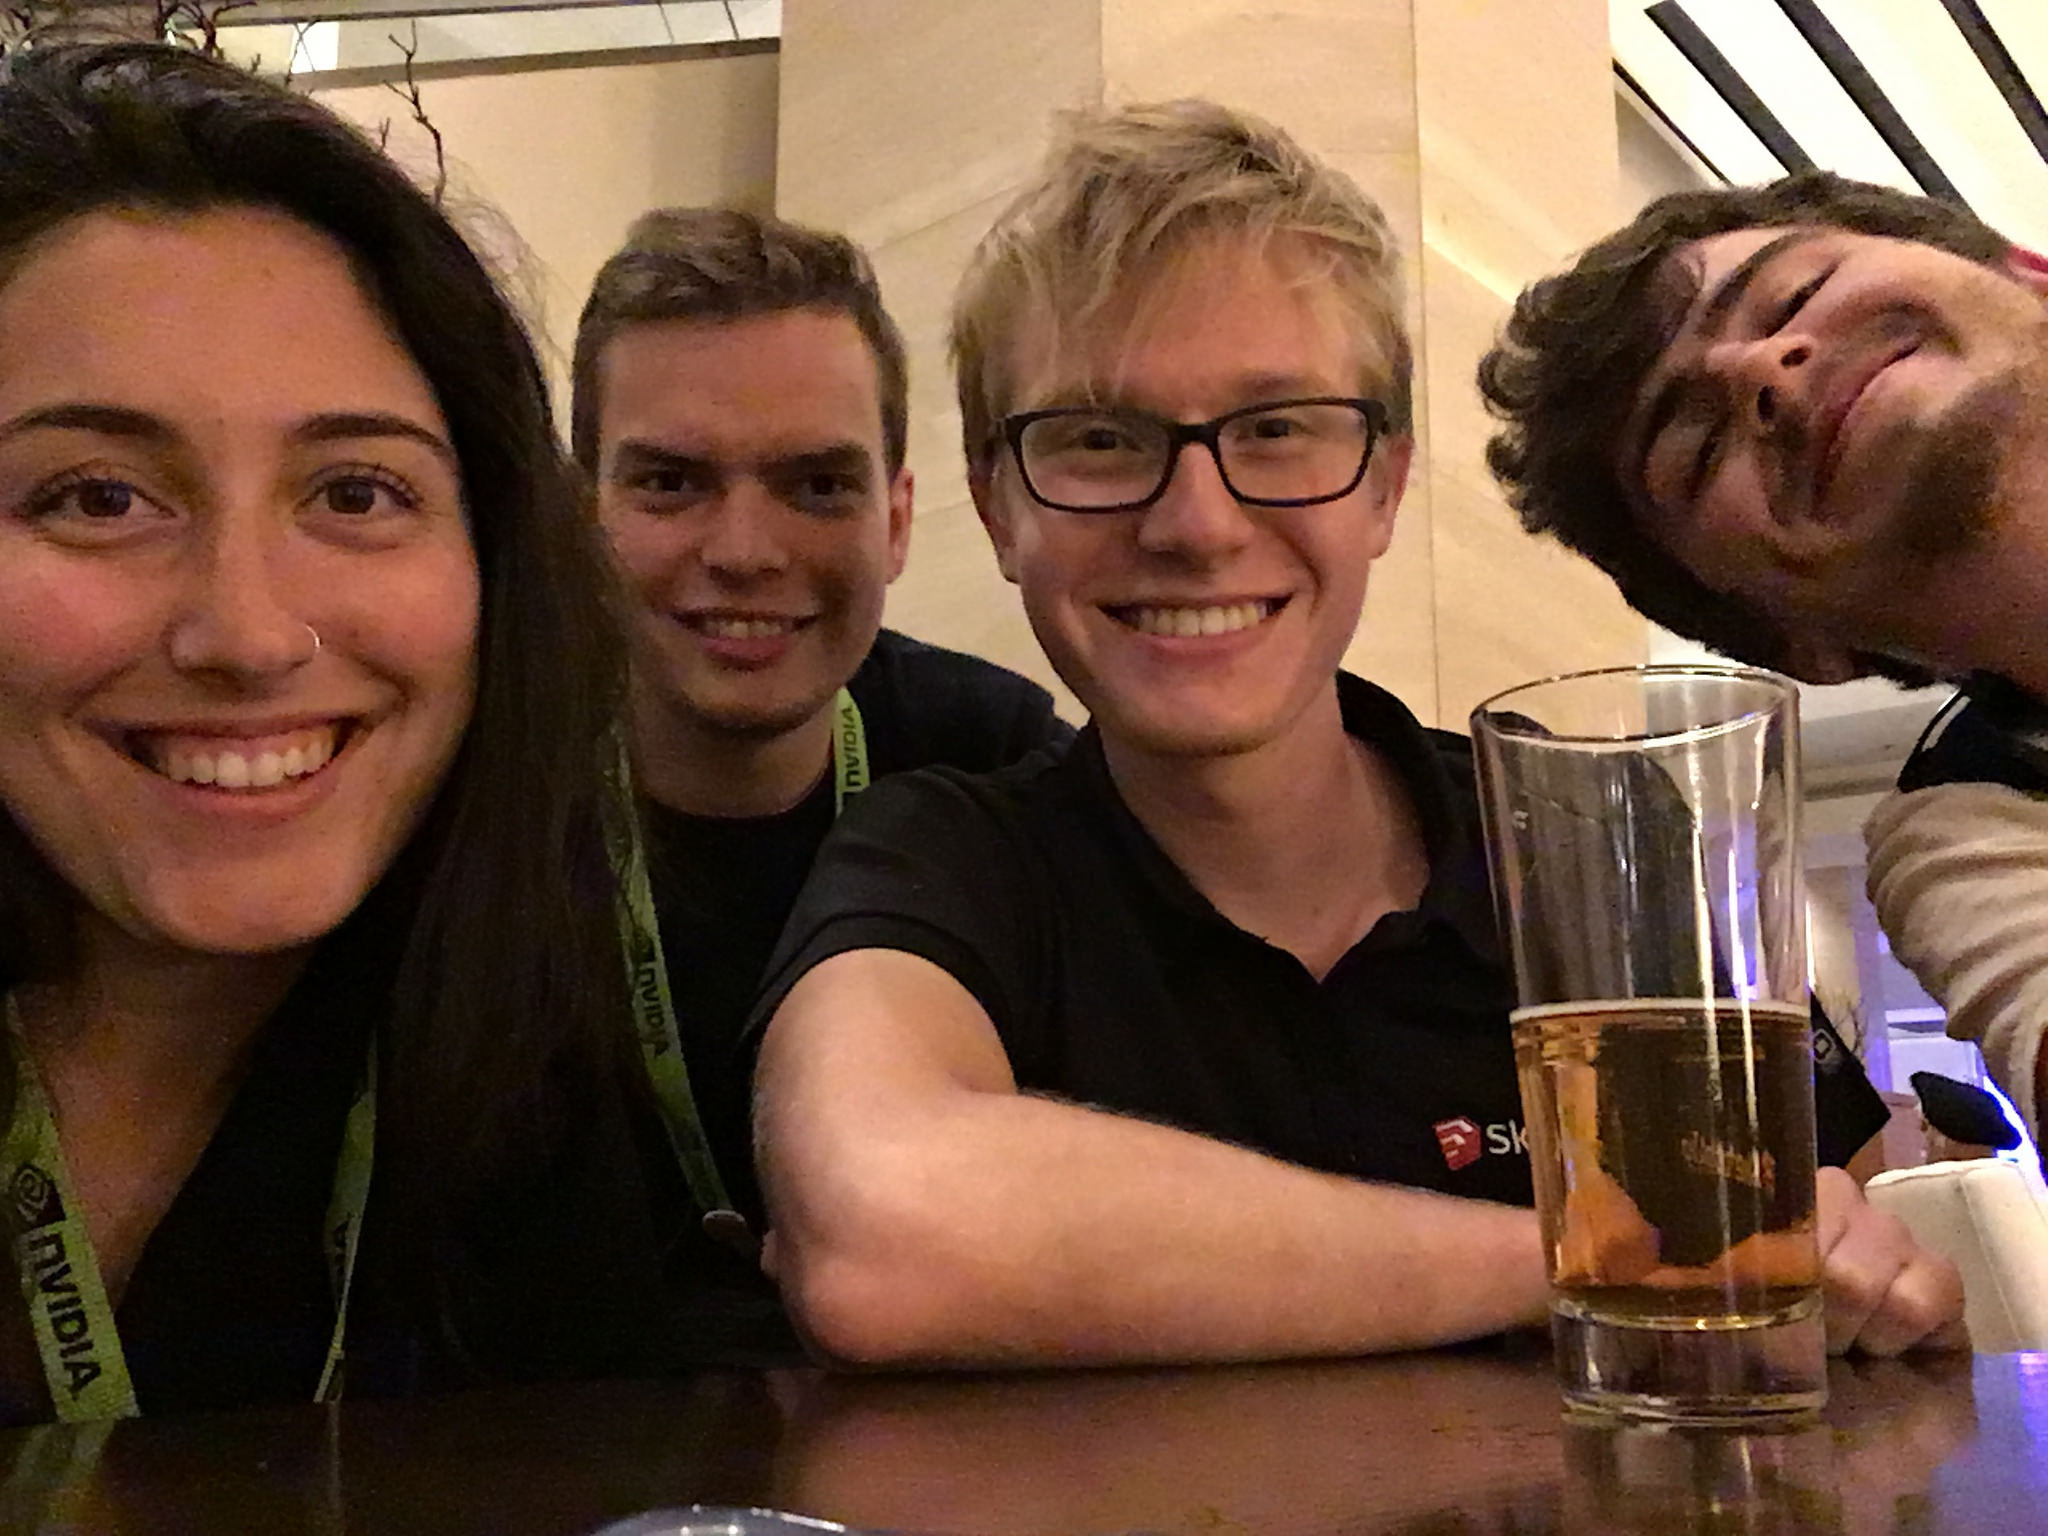
\includegraphics[width=\textwidth]{khronos_party}
	\caption*{Crashing the Khronos party.}
\end{figure}

\end{document}